\label{ch:desing}
\chapter{Diseño e Implementación}
\section{Propuesta de solución}
\label{sec:propuesta-sol} 
La propuesta para detectar fuga de información en aplicaciones Android, antes de
su publicación, consiste en proveer al desarrollador una herramienta para
análisis estático de flujos de información de la aplicación. Así, partiendo de
las anotaciones de seguridad que el desarrollador defina en el código fuente, se
verifica si la aplicación cumple con políticas de seguridad.\newline
% \textcolor{red}{Cómo sabe el desarrollador que información anota con nivel de
% seguridad bajo y con nivel de seguridad alto?}\newline
Los requerimientos iniciales para construir tal herramienta son: un lenguaje
tipado de seguridad que permita anotar código fuente Android, y el conjunto de
reglas que evaluarán las políticas de seguridad.\newline 
Al consultar literatura científica al respecto, se encuentran herramientas como
Jif \ref{JIF-Tool} y Joana \ref{JOANA-Tool}, especializadas en anotar código
Java, pero no código Android. Es decir, las anotaciones son válidas para clases
del lenguaje java estándar, pero no para clases específicas de la API de Android.

Si bien, ambas herramientas analizan flujos de información en aplicaciones Java,
y podrían ser extendidas para anotar código Android, sus técnicas de análisis y
forma de anotación son diferentes.
Por un lado, Jif es un lenguaje tipado de seguridad que basa su análisis en el
chequeo de tipos.
Por el otro, Joana es un framework basado en análisis de grafos de
dependencia, enfocado a precisión.\newline
Mientras Jif se basa un un modelo de anotaciones(DML), permitiendo la
implementación de aplicativos con políticas de seguridad; Joana sólo requiere
anotaciones para el nivel de seguridad de la información a analizar, en
aplicativos ya implementados.\newline
Adicionalmente, el modelo de anotaciones (DLM) de Jif, define  la lattice de
seguridad adecuada para las anotaciones en el código fuente, ofreciendo un
maduro sistema que además de evaluar políticas de confidencialidad, e
integridad, permite definir características de seguridad adicionales como
declasificación y endorsement.\newline
Acorde a los propósitos del presente trabajo, Jif ofrece los beneficios de un
lenguaje tipado de seguridad y un sistema  sólido  de anotaciones, facilitando
la definición de las propiedades de seguridad a verificar. 

Partiendo de Jif como el lenguaje tipado de seguridad, los retos subsiguientes
son: implementar el setup de Jif para Android e integrar un clasificador
para sources y sinks de Android.\newline 
El setup de Jif para Android consiste en implementar adaptaciones necesarias
a las clases de la API Android, de modo que, el compilador de Jif reconozca
anotaciones Jif en aplicaciones Android. Estas adaptaciones son necesarias
porque, aunque Jif permite extender al lenguaje Java, y en el fondo las clases
de la API Android están implementadas en Java, si no se cuenta con una versión
Jif de tales clases, el compilador de Jif no tiene como reconocerlas.\newline
% , y por
% tanto, no admite anotaciones en programas que usen esas clases(aplicativos
% Android).\newline
% en implementar las adaptaciones necesarias
% para que el lenguaje JIF reconozca código de la API de Android, y admita
% anotaciones JIF dentro de código Android, pues aunque en esencia el código
% Android es código Java, JIF no tiene como saberlo. 
Con la integración de un clasificador de sources y sinks para Android al sistema
de anotaciones de JIF, se provee información necesaria para construir las
políticas de seguridad. Porque, al conocer qué código de la API de Android,
es considerado como source o como sink, se tiene el criterio para decidir su
anotación.
% Permitiendo conocer el nivel de seguridad con que deben ser
% anotados el código tanto de la API como el código del aplicativo a
% analizar.\newline
%Si el desarrollador no sabe que es source y que es sink, cómo sabe que nivel
% de seguridad anotar durante la implementación de la versión JIf que va a
% evaluar 
% La figura \ref{fig:desingInteger} expone los elementos necesarios para construir la
% herramienta de análisis.

Básicamente, se requiere un módulo que extienda las clases en JIF para que el
lenguaje reconozca código de la API Android(\emph{Android Jif Setup}), más un
módulo que integre el clasificador de sources y sinks para Android(\emph{Sources
y Sinks}). 
Ambos módulos deben tener comunicación con el módulo que evalúa las
políticas de seguridad \emph{verificador de políticas}, que en esencia es el
compilador de Jif.\newline
% s decir, para que admita anotaciones dentro del código Android: Setup extended JIF classes.
% Un módulo que integre el clasificador de sources y sinks de Android al
% sistema de anotaciones en JIF:  Android Sources and Sinks. Adicionalmente, se
% requiere un modulo que evalúe las políticas de confidencialidad, Checking
% Rule Sets, que debe tener comunicación con los módulos anteriormente descritos.
% Adicionalmente, la figura \ref{fig:desingInteger} ilustra que la herramienta
Adicionalmente, la herramienta
debe recibir como entrada el código fuente de la aplicación, debidamente
anotado por el desarrollador. De modo que el desarrollador defina las políticas
de seguridad a evaluar. A partir de tales anotaciones, la herramienta de
análisis verifica si los flujos de información del aplicativo, cumplen con la
política de seguridad expresada a través sus anotaciones, y retorna los
resultados del análisis.

Habiendo realizado las extensiones necesarias, se espera contar
con una herramienta de análisis de flujo de información, para aplicativos Android,
mediante el sistema de anotaciones de Jif.

% \begin{figure}[t!]
% 	\begin{center}
% 	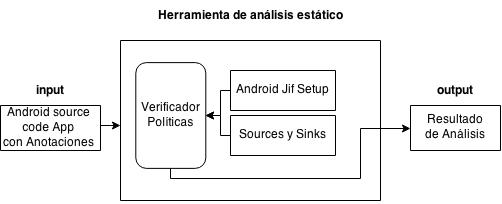
\includegraphics[width=10cm]{desing3-integration.jpg} 
% 	\end{center}
% 	\caption{Herramienta de análisis estático  }
% 	\label{fig:desingInteger}
% \end{figure}

% \begin{figure}[t!]
% 	\begin{center}
% 	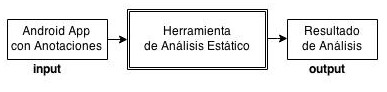
\includegraphics[width=9cm]{desingInOut-3.jpg}
% 	\end{center}
% 	\caption{Herramienta de análisis estático. Ilustra entradas y salidas
% 	esperadas}
% 	\label{fig:desing1}
% \end{figure} 

%color-question para Martín
% \textcolor{blue}{ \textit{P: desde este parrafo hasta el final de la sección,
% está bien dejar esa información así, o sencillamente la podemos omitir?}}\newline
% Luego, la estrategia de evaluación, consiste en verificar si la herramienta
% identifica pérdida de información mediante detección de flujos implícitos. Esto
% debido a que, como se menciona en la descripción del problema, parte importante
% de las propuestas para detección de fuga de información en aplicaciones Android,
% hacen data-flow analysis aplicando técnicas de análisis tainting, y en contraste
% con las técnicas de análisis de flujo de información, las técnicas de análisis
% tainting no necesariamente consideran flujos implícitos. Por tanto, al estar
% basada en JIF, cuyo enfoque de análisis es precisamente flujo de información, se
% esperaría que la herramienta propuesta esté en capacidad de reconocer flujos
% implícitos.
% 
% % Se esperaría que: al realizar análisis de flujo de información aplicando
% % técnicas Security-Typing, la herramienta propuesta, esté en capacidad de
% % reconocer flujos implícitos.\newline
% % Más específicamente, se puede tomar el conjunto de aplicaciones utilizadas como
% % casos de prueba para la detección de flujos implícitos en
% % DroidBench\cite{DroidBenchBenchmarks}, el benchmark de Flowdroid, y analizarlas
% % con la herramienta propuesta.\newline
% 
% Más específicamente, se puede partir de DroidBench\cite{DroidBenchBenchmarks},
% el benchmark de Flowdroid[\ref{FlowDroid-Tool}], tomar el conjunto de
% aplicaciones con que prueban la detección de flujos implícitos, y analizarlas
% con la herramienta propuesta.\newline
% Finalmente estos resultados serían
% comparados con los obtenidos mediante otras herramientas para análisis de fuga
% de información en aplicaciones Android.
% 
% En este orden de ideas, la evaluación de la herramienta propuesta está enfocada
% en: medir recall frente a la detección de flujos implícitos, es decir, medir que
% no genere falsos negativos ante la existencia de fugas de información,
% provenientes de flujos implícitos.\newline
% 
% 






\section{Limitaciones técnicas}
\label{sec:limitaciones}
\textcolor{blue}{P: estás limitaciones técnicas realmente deben ir aquí?}
Como parte del diseño de la solución, se inicia con una etapa exploratoria. En
esta se anotan manualmente varias aplicaciones de Android, y se identifican
limitaciones del lenguaje Jif para anotar código de la API de Android.
Tales limitaciones son adicionales a las características del lenguaje Java no
reconocidas por Jif, a continuación se describen tanto las encontradas, como las
especificadas en el manual de referencia de Jif.

-\textit{Características del lenguaje Java no soportadas por jif}\newline
Si bien, el sistema de anotaciones de Jif hace extensiones al lenguaje java,
permitiendo la evaluación de políticas de confidencialidad e integridad para
aplicativos implementados en dicho lenguaje, el manual de referencia de Jif
precisa las características del lenguaje Java no soportadas\cite{jifRef}. Estas
son:
\begin{itemize}
  \item nested classes: clases que son definidas dentro de otras clases.
  \item initializer blocks: bloques de código declarados dentro de la clase pero
  sin pertenecer a ningún método, dependiendo de si se trata de static
  initialization blocks, su código es el primero en ejecutarse, una vez se
  carga la clase; o si se trata de instance initialization blocks, su código se
  ejecutan cada vez que se crea una instancia de la clase.
\item threads.
\end{itemize} 
Partiendo de estas precisiones, aplicaciones Android que presenten tales
características son excluidas del grupo de aplicaciones a analizar(conjunto de
aplicaciones evaluables) mediante la herramienta propuesta.

% Adicional a las limitaciones de jif frente a características propias del
% lenguaje Java, tras experimentar la anotación manual de una serie de
% aplicaciones Android, se identifican varias limitaciones técnicas para la
% anotación de de las mismas. Entre las limitaciones identificadas están:\newline 

- \textit{Soporte para sobreescritura de métodos}\newline 
En la construcción de aplicaciones Android, según el componente que se esté
implementando(activities, content providers, receivers, services), se requiere
sobreescribir métodos de la clase que extienda el componente. Así, cuando se
define un componente tipo Activity, que debe extender de la clase Activiy.java, 
se sobreescriben métodos como Oncreate. Cada que se sobreescribe
un método se utiliza el statement @Override, con el cual se informa al
compilador de Java que el método es sobreescrito. No obstante, al implementar la
versión Jif de aplicaciones Android con dicho statement, el compilador de Jif
no lo reconoce. La dificultad que se presenta está en el reconocimiento del
statement(carácter @ y clase Override), y no en la sobreescritura de métodos,
puesto que Jif soporta tal característica. El soporte para la sobreescritura de
métodos es confirmado con una sencilla prueba, anotando la clase Activity.java
del framework Android (con un único método, el método Ocreate), e implementando
la versión Jif de una aplicación Android que extiende de tal clase, en la cual
se define una actividad y sobreescribe el método Oncreate.
Cuando se comenta la sentencia @Override, el compilador de Jif identifica la
sobreescritura del método y reporta comentarios para el flujo de información.\newline 
Al investigar el por qué Jif no reconoce tal sentencia, se encuentra que dentro
de las clases Java estándar soportadas por el compilador de Jif, no está
contenida la clase java.lang.Override.\newline
Las clases Java estándar pertenecientes a los paquetes io, lang, math, net y
sql; para las que el compilador Jif brinda soporte, vienen implementadas con
anotaciones en el directorio sig-src, directorio que forma parte de la
distribución del compilador de Jif con que se esté trabajando.\newline
Una alternativa para permitir el análisis de flujo de información entre métodos
que se sobreescriben, es comentar las líneas del programa que contengan la
sentencia @Override, puesto que, al no ser reconocida por el compilador de Jif,
es la generadora de errores de compilación.

- \textit{Casting entre tipos EditText y View}\newline
El framework de Android cuenta con diferentes clases para manejar las interfaces
gráficas que presenta al usuario, entre las cuales se encuentran EditText y
View. View es la clase principal para la creación de widgets, necesarios para la
implementación de componentes interactivos en las interfaces de usuario(UI).
EditText permite adicionar campos de texto editables en UI. El casting entre los
tipos de datos que representan ambas clases, se hace cuando la aplicación debe
procesar datos provenientes de campos en las interfaces del usuario, por ejemplo
como se observa a continuación:
\begin{lstlisting}
EditText editPassword = (EditText)findViewById(R.id.password);
String password = editPassword.getText().toString();
\end{lstlisting}
la interfaz de usuario(que es de tipo View) contiene un campo R.id.password, y
para manipular la información que almacena, debe ser de tipo EditText, siendo
necesario un casting de tipo View a tipo EditText. La dificultad que se presenta
con este tipo de casting es que para el sistema de anotaciones de jif no es
válido. Luego de probar con la anotación manual de ambas clases, tratando de
dar soporte a este tipo de casting, sin obtener resultados satisfactorios, se
opta por ``simular'' estos casos, es decir, si el tipo de dato de una variable
es de tipo EditText, se crea una variable tipo String con un valor determinado,
así se omite el casting y se puede analizar el flujo de información.

- \textit{Clase nested R}\newline
El framework de Android utiliza identificadores para hacer referencia a recursos
utilizados por la aplicación, recursos como strings, widgets y layouts, tales
identificadores son autogenerados en la clase R.java, allí cada recurso es
descrito como una clase individual. Al tratarse de una clase nested, la clase R
no puede ser anotada con jif. Esto puede solucionarse implementando una
versión Jif generalizada de la clase R, que contenga los recursos utilizados en
una aplicación, definidos como variables y no como clases.

% - \textit{Sources y Sinks}\newline
% En los preliminares para el diseño de la solución se propone utilizar SuSi
% para clasificar los sources y sinks en las aplicaciones a analizar, sin embargo, partir del
% extenso conjunto de sources y sinks, clasificados por SuSi para la API de
% Android, implica una mayor complejidad en el análisis, puesto que, en un
% aplicativo todo el código que le conforma puede hacer parte de sources o de
% sinks. Adicional a lo complejo que se puede tornar el análisis, los sources y
% sinks a considerar deben depender de la política de seguridad a evaluar. En ese
% orden de ideas, resulta más viable tomar un subconjunto del listado proveído por
% SuSi, partiendo de los sources y sinks que evalué la política de seguridad que
% se defina.

- \textit{Enhanced for loop} \newline
Además de soportar la estructura de control for, el lenguaje Java permite el uso
de enhanced for, que es utilizado para simplificar la iteración en arrays y
colecciones, por ejemplo:
% \begin{lstlisting}
% char c[] = imei.toCharArray();
% for (int i = 0; i < c.length; i++) {
% 	obfuscated += c[i] + "_";
% }          
% \end{lstlisting}  
\begin{lstlisting}
for(char c : imei.toCharArray())
obfuscated += c + "_";
\end{lstlisting}
A diferencia de Java, Jif no soporta el enhanced for.\newline
Debido a que ambas sentencias de control son equivalentes, la solución que se
propone para poder analizar flujo de información en los aplicativos Android que
contengan dicha estructura de control, es generar el equivalente del programa
haciendo uso del for, de este modo se cambia la sintaxis sin afectar la lógica
del aplicativo a analizar.

- \textit{Otras limitaciones} \newline
Adicional a las limitaciones descritas anteriormente, para las cuales se propone
una solución, se identifica que Jif no soporta la sintaxis utilizada para
definir estructuras de datos HashMaps, LinkedList y Sets, que en Java se definen
de la siguiente manera:
\begin{lstlisting}
Map<String,String> hashMap = new HashMap<String, String>();
List<String> listData;
Set<String> phoneNumbers = new HashSet<String>();
\end{lstlisting}
Jif tampoco permite la definición de interfaces como argumentos de un método. El
siguiente fragmento de código  en una aplicación Android, muestra la definición
de una interfaz pasada como parámetro al método setOnClickListener.
\begin{lstlisting}
   Button button1= (Button) findViewById(R.id.button1);
   button1.setOnClickListener(new View.OnClickListener() {
   ...
   .....}  });
\end{lstlisting}
En estos casos, la dificultad está en encontrar una sintaxis que permita obtener
la versión equivalente del programa que las contenga. A lo que se suma, la falta
de documentación disponible para solventar los mismos. En consecuencia, se omite
del conjunto de aplicaciones evaluables, aplicaciones Android que requieran en
su implementación las estructuras de datos descritas.\newline

%- \textit{Paso de statements dentro de los argumentos de un método
%(\{\}):}\newline

\section{Diseño de la solución}
Como se describe en la propuesta de solución \ref{sec:propuesta-sol}, el
diseño ideal para contribuir con la solución del problema es: una herramienta
que contenga el setup de Jif para Android, e integre un clasificador de
sources y sinks, de tal manera que la herramienta permita evaluar el control de
flujo de información en aplicativos Android. Así, mediante anotaciones Jif en el
código de su aplicación, el desarrollador define la política de seguridad a evaluar.

Sin embargo, para efectos de esta tesis se limita el Setup de Jif, partiendo de
una política de seguridad específica. De este modo, el diseño se centra en
soportar un conjunto reducido de clases de la API de Android, y en incluir un
conjunto específico de sources y sinks de acuerdo a una política de seguridad
establecida. Ese conjunto de sources y sinks, se toma del listado de sources y
sinks proveído por SuSi \ref{sec:susi}.\newline 
Adicionalmente para aspectos de evaluación, se incluye el diseño de un anotador
que anota automáticamente el conjunto de aplicativos a analizar acorde a la
política de seguridad que se evalúa. La figura \ref{fig:desingReal} muestra el
esquema del diseño.
\begin{figure}[t!]
	\begin{center} 
	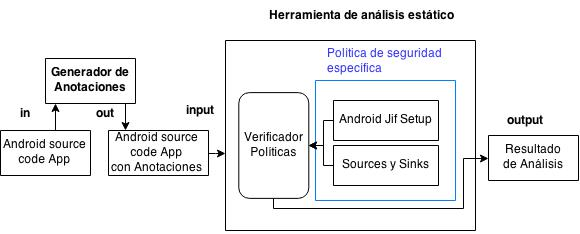
\includegraphics[width=11cm]{desing3Real.jpg} 
	\end{center}
	\caption{Diseño herramienta de análisis estático}
	\label{fig:desingReal}
\end{figure}

% En los preliminares para el diseño de la solución se consideró la siguiente
% opción: Anotar un conjunto de clases de la API de Android mediante el sistema de
% anotaciones de Jif, de modo que el compilador de Jif reconociera clases propias
% de esa API, y por tanto, permitiese el análisis de flujo de información a través
% de estas. Habiendo asegurado el reconocimiento a un
% conjunto de clases de la API de Android, era tarea del desarrollador implementar
% la versión Jif del aplicativo a evaluar.
% 
% Si bien, con dicha opción de diseño se aporta para que el desarrollador
% Android evalúe flujos de información en su aplicación, mediante Jif; también se
% incrementa su carga de programación, puesto que, al delegarle la anotación de la
% aplicación a analizar, este debe pensar dos versiones. La versión .java, donde
% utiliza los métodos proveídos por la API Android para definir las
% funcionalidades de su aplicación; y la versión .jif, donde define las
% anotaciones pertinentes para evaluar flujos de información; tarea para la cual,
% se requiere un conocimiento previo del sistema de anotaciones de Jif y la
% implementación de aplicaciones haciendo uso de las mismas.
% 
% En consecuencia, se opta por un diseño que reduzca la carga de programación
% del desarrollador, durante el análisis del aplicativo.\newline 
% El diseño de solución consta de dos elementos fundamentales: anotaciones a la
% API de Android, más el anotador que genere la versión Jif del aplicativo a
% analizar, acorde a una política de seguridad previamente definida.\newline 
% Ambos elementos son complementarios, puesto que, por más que se genere la
% versión Jif del aplicativo a analizar, si el compilador no reconoce clases
% específicas de la API que allí se usan, .jif no puede ser compilado.

Así, (1) se parte definiendo la política de seguridad a evaluar
\ref{subsection:politica}, (2) se toman a consideración elementos influyentes
para verificar el cumplimiento de la política mediante Jif
\ref{subsec:consVerPol}, y finalmente, teniendo en cuenta (1) y (2), se definen
los lineamientos de anotación \ref{subsec:linemientos}, donde se establece el
esquema tanto para las anotaciones requeridas en la API como para las
anotaciones de los aplicativos a analizar(lineamientos del anotador).

\subsection{Definición de la política de seguridad}
\label{subsection:politica}
Detectar si una aplicación Android(perteneciente al conjunto evaluable) presenta
flujos de información entre, información con nivel de seguridad alto e
información con nivel de seguridad bajo.\newline
Detectando fugas de información catalogada con nivel de seguridad alto, vía:
canales creados durante el control de flujo del programa(flujos implícitos),
mensajes de texto y mensajes de Log.\newline 

\subsection{Consideraciones para verificar el cumplimiento de la política
mediante Jif} 
\label{subsec:consVerPol}
Teniendo definida la política de seguridad a verificar se describe: cuál es la
información considerada con nivel de seguridad alto; cuáles son los canales que
muestran información con nivel de seguridad bajo; cuál es el punto de entrada
para el análisis de la aplicación(diferencia entre una aplicación Android y una
aplicación Java convencional); qué se espera del desarrollador si la aplicación
a analizar requiere excepciones tipo Runtime; qué se asume para evaluar el flujo
de información; y cómo es el acceso a métodos que deben ser
sobreescritos.\newline
Todos, elementos relevantes para proponer un esquema de anotación.

\textit{Información considerada con nivel de seguridad alto}\newline
Para verificar el cumplimiento de la política de seguridad a evaluar se parte de
un conjunto de sources, caracterizados por dar a conocer
información del usuario, considerada como privada o sensible. Los métodos que integran
el conjunto de sources son: getDeviceId, getSimSerialNumber, findViewById,
getLatitude, getLongitude y getSubscriberId. Adicional a estos métodos, se
incluye el tipo de dato EditText, si y sólo si, el campo UI al que referencia
corresponde a un campo tipo textPassword, es decir, un campo que almacena
contraseñas.\newline 
Este conjunto de sources es tomado del listado proveído por el clasificador SuSi
\ref{sec:susi}.

\textit{Canales que muestran información con nivel de seguridad bajo}\newline
La información enviada a través de mensajes de texto y la información conocida
tanto a través de mensajes de Log, como a través de canales generados por el
control de flujo del programa, tiene en común que debe poderse conocer por
terceros.
En consecuencia, se considera que estos canales deben dar a conocer información
con nivel de seguridad bajo.\newline En el caso de mensajes de texto y mensajes
de Log, se hace referencia específicamente a las clases Log y SmsManager de la
API de Android.

\textit{Diferencia entre una aplicación Android y una aplicación Java
convencional}\newline 
En esencia, una aplicación Android es una aplicación Java con interfaces
descritas en XML, que para ser ejecutada necesita del framework de Android,
porque este le provee acceso al hardware del dispositivo y funcionalidades del
sistema.\newline 
Por otro lado, Jif permite hacer seguimiento al flujo de información de una
aplicación Java, extendiendo el lenguaje mediante labels de seguridad.\newline
Para analizar flujo de información de una aplicación Android mediante
Jif, es importante mencionar que mientras una aplicación Java convencional
cuenta con un único punto de entrada para iniciar su ejecución, esto es, la
clase principal donde se implementa el método main; una aplicación Android puede
tener más de un punto de entrada, generados a partir de los diferentes tipos de
componentes que le integren(Activity, Service, Content Provider y Broadcast
Receiver). La necesidad de interacción del usuario para activar tales puntos de
entrada varía acorde al tipo de componente, así, en el caso de componentes tipo
Activity su ejecución sólo inicia hasta que el usuario interactúe con la
actividad, y para manejar dicha interacción, la API Android provee el método
OnCreate. De otro modo, componentes tipo Service y Broadcast Receiver, inician
su ejecución a través de los métodos OnStartCommand y OnReceive,
respectivamente, sin necesidad de interacción del usuario.\newline 
{ \color{black} {Teniendo en cuenta lo anterior, se asume que la aplicación a
evaluar tiene un único punto de entrada, que depende del tipo de componente que
implemente.} }

\textit{Chequeo de excepciones tipo Runtime}\newline
En lenguaje Java las excepciones tipo Runtime tales como NullPointerException, no
son verificadas a tiempo de compilación, sin embargo, buscando evitar la
generación de canales encubiertos mediante las mismas, Jif si las verifica. 
En consecuencia, si un programa requiere excepciones NullPointerException,
ClassCastException y/o ArrayIndexOutOfBoundsException, el programador debe
declararlas en el programa, de lo contrario, el compilador de Jif genera error.
Para las aplicaciones a analizar, se espera que el desarrollador haya
especificado las excepciones necesarias.

\textit{Evaluación del flujo de información}\newline
Para evaluar el flujo de información, se asume que todos los métodos definidos
en la clase serán invocados, y por tanto, todos son incluidos en el análisis.\newline 
Esta decisión de análisis busca evitar el paso inadvertido de flujos de
información, generados por omisión.

\textit{Acceso a métodos de sobreescritura.}\newline
Los métodos de las clases Activity, Service y BroadcastReceiver, son métodos
que se pueden sobreescribir, todo programa Android que extienda de tales clases
debe poder utilizarlos.

\subsection{Lineamientos de anotación}
\label{subsec:linemientos}
Para verificar el cumplimiento de la política de seguridad
establecida \ref{subsection:politica} mediante el sistema de anotaciones de Jif,
se requiere: (a) definir los elementos básicos de anotación, (b) definir
las anotaciones necesarias para la API de Android y (c) definir los
criterios de anotación para los aplicativos a analizar, tales 
criterios se sintetizan en un anotador.

%\textbf{(a)Elementos básicos de anotación}\newline
\subsubsection{(a) Elementos básicos de anotación}
En \ref{subsec:consVerPol} se definió qué \textit{Canales muestran
información con nivel de seguridad bajo} y cuál es la \textit{Información
considerada con nivel de seguridad alto}. Ahora, para anotar la información
catalogada con uno u otro nivel de seguridad, de modo que, partiendo de tales
anotaciones se evalué la existencia de flujos de información entre información
con nivel de seguridad alto e información con nivel de seguridad bajo, lo primero
que se debe definir es quién es la autoridad de los programas y cuáles son los
labels de seguridad.\newline
Conceptos y términos implicados en la sintaxis de anotación Jif, se
encuentran en la sección de background \ref{sssec:JifSintax}.

Principal \emph{Alice}\newline
aprovechando que Jif ya trae una serie de principals establecidos, se define que
la autoridad máxima es el principal Alice. Este principal tendrá todo el poder
para actuar sobre aspectos de los programas.

Label de seguridad \emph{\{Alice:\}}\newline
este label indica que la información tiene nivel seguridad alto, es decir, que
se trata de información sensible o privada.\\
Variables con nivel de seguridad alto deben ser anotadas con tal label de
seguridad, porque esté específica que sólo el dueño de la información(Alice)
puede acceder a la misma. 

Label de seguridad \emph{\{\}}\newline
este label indica que la información tiene nivel de seguridad bajo, es decir,
información de conocimiento público.

\subsubsection{(b) Anotaciones a la API de Android}
%\textbf{(b)Anotaciones a la API de Android}\newline

\begin{figure}[h!]
	\begin{center}
	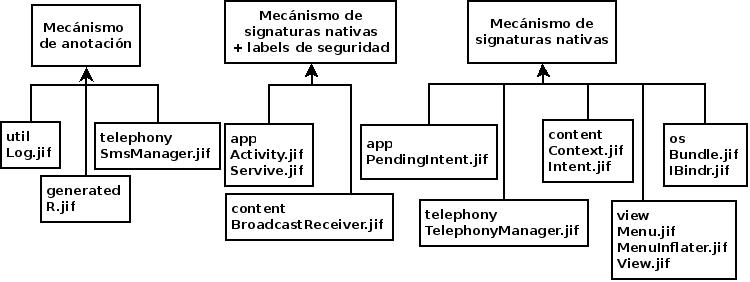
\includegraphics[width=12cm]{annotationsMechanims.jpeg}
	\end{center}
	\caption{Mecanismos de anotación para clases de la API.}
	\label{fig:annotationsMechanims}  
\end{figure}

- Anotaciones para \textit{Canales que muestran información con nivel de
seguridad bajo}: para controlar el flujo de información que se envía hacia
\textit{Canales que muestran información con nivel de seguridad bajo}, es
necesario anotar la definición de los métodos de las clases Log y SmsManager de
la API Android, de manera tal que se controle el nivel de seguridad de los
argumentos con que se invocan.\newline
Tomando como ejemplo el método sendTextMessage de la clase SmsManager, mediante
el cual se envían mensajes de texto:
\begin{lstlisting}
sendTextMessage(String destinationAddress, String scAddress, 
String text, PendingIntent sentIntent, PendingIntent deliveryIntent)
\end{lstlisting}

Se tiene que el parámetro \emph{text} es el que recibe la información a mostrar,
y por tanto esa información debe ser pública.\newline 
Por consiguiente, en la definición del método el label de seguridad del
argumento(AL) correspondiente a la información a mostrar(logs) o la información
a enviar(sms), se anota con el label de seguridad bajo(label público\{\}). Con
esto se garantiza que la información se muestra o envía, si y sólo si el nivel
de seguridad del argumento con que se invoca el método es público. Por ejemplo,
si el método se invoca con información anotada con label de seguridad alto, se
genera error en la compilación del programa que le llama.\newline 
El resto de argumentos del método se anotan con label de seguridad \{Alice:\},
puesto que esa información puede ser pública o privada.\newline
En el caso del BL al anotarlo con el label \{Alice:\}, se permite que el método
sea invocado desde cualquier punto de un programa. 
Para el resto de labels se dejan los que Jif genera por defecto.\newline
% cualquier punto de un programa que sea igual o menor de restrictivo que el
% principal Alice, esto se traduce en que podrá ser invocado desde cualquier punto
% de un programa, lo cual es correcto porque lo que se busca el evitar que se
% envíe información considerada con nivel se deguridad alto y no, evitar que el
% método sea utilizado. Poner ejemplo XXXX?\newlie
Continuando con el ejemplo del método sendTextMessage y aplicando lo
anteriormente descrito, este método se anota de la siguiente manera:
\begin{lstlisting}
sendTextMessage{Alice:}(String{Alice:} destinationAddress, 
	String{Alice:}scAddress, 
	String{} text, 
	PendingIntent{Alice:} sentIntent,
	PendingIntent{Alice:} deliveryIntent) { }
\end{lstlisting}

- Anotaciones para métodos de sobreescritura: en \ref{subsec:consVerPol},
también se definieron las clases de la API para las que se debe soportar el
\textit{Acceso a métodos de sobreescritura}(Activity, Service y
BroadcastReceiver). La anotación para la definición de tales métodos se basa en:
(1)reglas de Jif para la sobreescritura de métodos y (2)desde dónde pueden ser
invocados. (1)Jif exige que el nivel de seguridad del BL del método desde donde
se invoca el método a sobreescribir, no debe ser menos restrictivo que el BL de
la definición de tal método(privado es más restrictivo que público). (2) la
sobreescritura de métodos se debe poder utilizar desde aplicativos que extiendan
de las clases Activity, Service y BroadcastReceiver.\newline 
Para cumplir con (1) y (2), los métodos que requieren ser sobreescritos se
definen con BL público(\{\}). De este modo los aplicativos desde dónde se
invocan los métodos a sobreescribir deben tener igual BL.\newline
Por ejemplo, el método OnCreate de la clase Activity, se define de la forma:
\begin{lstlisting}
protected native void onCreate{}(Bundle savedInstanceState);
\end{lstlisting}

- Anotaciones a librerias de la API: 
adicional a las clases Log, SmsManager, Activity, Service y
BroadcastReceiver, es necesario soportar las librerías requeridas por estas,
para lo cual se utilizan signaturas nativas de anotación. Tales librerías son:
android.app.PendingIntent\\
android.telephony.TelephonyManager\\
android.content.Context\\
android.content.Intent\\
android.text.Editable\\
android.os.Bundle\\
android.os.IBinder\\
android.widget.EditText\\
android.widget.TextView\\ 
android.view.Menu\\
android.view.MenuInflater\\
android.view.View 

% Y para poder integrarlas al conjunto de clases reconocidas por el compilador
% de Jif, basta con recurrir a signaturas nativas. Mediante el uso de signaturas
% nativas es posible incluir clases Java ya existentes. Tal mecanismo consiste en
% implementa una versión Jif de las clase fuentes, en la qué sólo es necesario
% declarar constructores y cuerpo de los métodos a utilizar.
% 
% Ahora, para incluir clases Java ya existentes es posible recurrir a signaturas
% nativas, con las cuales se implementa la versión Jif de las clases fuentes, esto
% es, declarando constructores y cuerpo de los métodos a utilizar.
- Integración de clases de la API de Android a las clases reconocidas por el
compilador de Jif:\newline
Definidos los criterios de anotación para las clases de la API, a las cuales se
debe implementar su respectiva versión Jif, se definen los mecanismos a utilizar
para implementar tal versión. Además del mecanismo de anotación completa en que
se basa la implementación de aplicativos en Jif(mecanismo de anotación), el
compilador provee un mecanismo que permite reutilizar código de clases Java ya
existentes, para esto, se recurre a signaturas nativas. Así, se implementa una
versión Jif de una clase Java ya existente, en la que se declaran signaturas
nativas proveídas por Jif, constructor y métodos necesarios de la
clase(mecanismo de signaturas nativas).
Al mecanismo de signaturas nativas también se puede  adicionar labels de
seguridad(mecanismo de signaturas nativas más labels de seguridad).\newline
Para el presente caso y de acuerdo a los criterios de anotación previamente
establecidos las clases a implementar mediante uno u otro mecanismo, son
ilustrados en la figura \ref{fig:annotationsMechanims}.\newline

\subsubsection{(c) Anotaciones en los aplicativos a analizar}
%\subsubsection{Criterios de anotación para los aplicativos a analizar}
%\textbf{(c)Criterios de anotación para los aplicativos a analizar}\newline
% XXXPara evaluar los flujos de información de una aplicación Android, de modo que
% se verifique si cumplen con la política de seguridad definida
% \ref{subsection:politica}; es necesario implementar su respectiva versión Jif,
% esto implica que variables y métodos de la clase sean anotados haciendo uso del
% sistema de anotaciones de Jif.\newline 
% Ante esto, se propone un esquema de anotación enfocado a detectar flujos de
% información desde: información considerada con nivel de seguridad alto,
% hacia: canales considerados con nivel de seguridad bajoXXX.
Los elementos en que se fundamenta el esquema de anotación para el aplicativo a
analizar, son los siguientes:\newline 
Primero, como los \textit{Canales que muestran
información con nivel de seguridad bajo} están anotados desde la definición en
sus respectivas clases de la API, de modo que la información a mostrar(logs) o
enviar(msn) debe tener nivel de seguridad bajo(debe ser pública), en el esquema
de anotación del aplicativo no es necesario identificar tales canales, pues
estos ya están definidos desde la API. Lo que si se debe hacer desde el esquema
de anotación del aplicativo, es proveer los labels de seguridad adecuados a la
información con que se invocan tales canales.

Segundo, la anotación para la sobreescritura de métodos de la API, está definida
en las respectivas clases de la API, el esquema de anotación para la invocación
de los métodos a sobreescribir debe ser consecuentes con tales definiciones de
anotación.

Tercero, el esquema de anotación para el aplicativo a analizar parte de
los sources que se identifiquen en el mismo. Tales sources pertenecen al conjunto
definido en (\textit{Información considerada con nivel de seguridad alto}),
conjunto que está integrado por el tipo de dato EditText\footnote{Este tipo de
dato es considerado como source si y sólo si, el campo UI al que referencia
corresponde a un campo tipo textPassword, es decir, un campo que almacena
contraseñas.} y los métodos: getDeviceId, getSimSerialNumber, findViewById,
getLatitude, getLongitude y getSubscriberId.

Cuarto, se parte de los \textit{Elementos básicos de anotación} previamente
definidos. Así, una clase Android tendrá como principal( autoridad máxima) al
principal \emph{Alice}, y los labels de seguridad para anotar información con
nivel de seguridad alto y nivel de seguridad bajo son: \emph{\{Alice:\}} y
\emph{\{\}}, respectivamente.

\textbf{\textit{Estructuración del esquema de anotación}}\newline 
Para concretar el esquema con que se anotan los aplicativos a analizar, se
establece la finalidad(Objetivo de la anotación), qué se va a anotar(Elementos
del esquema), cómo se van a anotar tales elementos(Anotación de los elementos) y
finalmente se indica cómo aplicar el esquema de anotación(Pasos para aplicar el
esquema de anotación). Así:

\textit{Objetivo de la anotación}\newline
El esquema de anotación se centra en identificar si una clase contiene sources,
y verificar si los métodos de la clase influencian esa información, de modo que,
cuando la información sea enviada por canales con nivel de seguridad bajo, tenga
el nivel de seguridad adecuado.

\textit{Elementos del esquema}\newline
Para referenciar los elementos que se anotan mediante este esquema, se
establecen una serie de términos, así:\newline
- Variable source: una variable source es una variable que almacena
información proveída por algún elemento del conjunto de sources.\\
- Array source: un array source es un array que almacena información de
variables source.\\
- Método que se sobreescribe: hace referencia a métodos de la API android
que deben ser sobreescritos para la implementación del aplicativo, por ejemplo, el
método Oncreate que se sobreescribe al implementar componentes tipo
Activity.\\
- Método source: un método source es un método(definido dentro de la
clase) que cuando es invocado, contiene dentro de los parámetros de invocación, al menos
una variable source.\\
- Método no source: un método no source es un método(definido dentro de la
clase) que cuando es invocado, no contiene dentro de los parámetros de invocación,
variables source.

\textit{Anotación de los elementos}\newline
Fijados los elementos que se anotan, se define su respectiva forma de anotación.
Conceptos y términos implicados en la sintaxis de anotación Jif, se
encuentran en la sección de background \ref{sssec:JifSintax}.
Los labels de seguridad que no son anotadas mediante este esquema, son generados
automáticamente por Jif, acorde a los labels que estable por defecto para la
definición de variables, métodos y arrays, etc.

- Definición A: anotación de variable source.\newline 
\emph{java-type \{Alice:\} nameVar}\newline
como la información almacenada en una variable source es información con nivel
de seguridad alto(conjunto de sources), la variable debe tener un label de
seguridad que indique que su información es de alta confidencialidad. Al
anotarla con el label \emph{\{Alice:\}}, se está indicando que esa información
pertenece al principal \emph{Alice}, así, cuando se envíe hacia un canal
de seguridad bajo, da lugar a un flujo de información indebido(de nivel alto a
nivel bajo).

- Definición B: anotación de array source.\newline
\emph{java-type\{Alice:\}[ ]\{Alice:\} arrayName}\newline
debido a que un array source almacena información con nivel de seguridad alto,
se debe garantizar que sólo el principal dueño de la información pueda
conocer tanto items como tamaño del array. Esto se logra anotando con
label de seguridad \emph{\{Alice:\}} el \emph{BL} y \emph{SL}, labels de
seguridad para los elementos y tamaño del array, respectivamente.

- Definición C: anotación de método que se sobreescribe.\newline
El BL de un método a sobreescribir debe ser anotado con label de seguridad bajo
\{\}, puesto que en su respectiva definición en las clases de la API, han sido
definidas con ese BL.

- Definición D: anotación de método source.\newline 
\emph{java-type\{Alice:\}  methodName \{Alice:\}(java-type arg1\{Alice:\} ,,,
java-type argn\{Alice:\})}
Como un método source influencia información con nivel de seguridad alto(variable
source), se debe garantizar que sólo sentencias del programa que tengan nivel de
seguridad alto, puedan ser actualizadas con información proporcionada por el método.\\
Buscando hacer cumplir lo anterior, se anota con label de
seguridad \{Alice:\} el RTL y el BL del método.
Retomando la sintaxis jif para anotación de métodos:\newline 
\emph{java-type \{RTL\} methodName \{BL\} (java-type arg1\{AL\},,, java-type argn\{AL\}):\{EL\} }\newline
Al anotar \{RTL\} con \{Alice:\} se asegura que, si el método retorna un valor,
tendrá nivel de seguridad alto.\newline
Al anotar \{BL\} con \{Alice:\} se asegura que, los puntos del programa que
traten de ser actualizados tras el llamado del método(por ejemplo variables, o
resultados de condicionales) deben tener un \underline{pc} con nivel de
seguridad alto.\newline
Para el caso de los AL, labels de seguridad de los argumentos, el sistema de
anotaciones de Jif exige que los AL con que se invoca el método, deben ser igual
o menor de restrictivos que los AL con que se define el método. 
Por otro lado, se tiene certeza de que uno de los argumentos con que se llama el
método tiene AL con nivel de seguridad alto(pues ese fue el criterio con que
se clasificó al método como source), pero el resto de parámetros puede tener AL
alto o bajo, entonces para garantizar que el método pueda ser invocado bajo
tales condiciones, los AL para los argumentos del método son anotados con
label \{Alice:\}.

- Definición E: anotación de método no source.\newline
\emph{methodName \{\} (java-type arg1\{Alice:\},,, java-type argn\{Alice:\})}\newline
Como el método no recibe la variable source, el nivel de seguridad de las
sentencias del programa que se actualicen con la información del método puede
ser bajo. Ahora,  si en el cuerpo del método se define o actualiza información
con nivel de seguridad alto(información global), tales sentencias deben tener
nivel de seguridad alto.
Anotando el BL con label {\{\}}, se respeta tal condición puesto que,
el BL se ve afectado cuando el cuerpo del método tiene información con mayor
nivel de seguridad, obligando a que las sentencias a actualizarse con la
información del método tengan nivel de seguridad alto.\newline
Para el caso de los AL, labels de seguridad de los argumentos, el sistema de
anotaciones de Jif exige que los AL con que se invoca el método, deben ser igual
o menor de restrictivos que los AL con que se define el método. Anotando los AL
de la definición del método con label \{Alice:\}, se cumple tal restricción ya
que el método es invocado con parámetros cuyo nivel de seguridad es bajo.

\textit{Pasos para aplicar el esquema de anotación}\newline
Partiendo de las anteriores definiciones, los pasos para la anotación son los
siguientes:\newline
(1) Identificar variables source de la clase. Si se encuentran variables sources
continuar con los pasos (2) a (11), sino, continuar con pasos: (3), (6), (9) y
Aplicar Definición E a los métodos que no se sobreescriben\footnote{Como no se
identifican sources, la anotación de método no source(Definición E) es
aplicable para los métodos que no se sobreescriben.}.
(2) Identificar arrays sources de la clase.
(3) Identificar el total de métodos de la clase.\newline
(4) Del total de métodos listar los métodos source.\newline
(5) Del total de métodos listar los métodos no source.\newline
(6) Del total de métodos listar los métodos a sobreescribir\newline
(7) Aplicar Definición D a listado del paso(4).\newline
(8) Aplicar Definición E a listado del paso (5).\newline
(9) Aplicar Definición C a listado del paso (6).\newline
(10) Aplicar Definición B a listado del paso (2).\newline
(11) Aplicar Definición A a listado del paso (1).

Para automatizar estos pasos, se debe implementar un generador de
anotaciones(prototipo de anotación). Que reciba como entrada el código fuente de
la aplicación Android(perteneciente al conjunto evaluable), y retorne su
respectiva implementación en Jif, versión que contiene las anotaciones para
evaluar la política de seguridad definida.\newline
La figura \ref{fig:desingSolution}, ilustra las entradas y salidas
esperadas.\newline
Luego la versión obtenida se evalúa con el compilador de Jif.
% \textit{Entradas y salidas del anotador}.
% Las definiciones y pasos para la anotación del aplicativo a analizar, descritas
% anteriormente, se condensan en un anotador. El cual debe recibir como entrada el
% código fuente de la aplicación Android(perteneciente al conjunto evaluable),
% para retornar su respectiva implementación en Jif, versión que contiene las
% anotaciones para evaluar la política de seguridad definida. Tal como se ilustra
% en la figura \ref{fig:desingSolution}\newline 
% Luego la versión obtenida se evalúa con el compilador de Jif.
\label{subsec:anotador}
\label{subsec:pasosSol}
\begin{figure}[t!]
	\begin{center}
	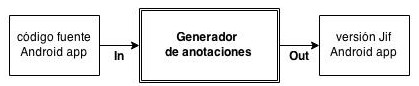
\includegraphics[width=10cm]{desingSolution2.jpg}
	\end{center}
	\caption{Entradas y salidas para el generador de anotaciones.}
	\label{fig:desingSolution} 
\end{figure}

% \subsection{Anotaciones a la API de Android}
% \label{subsec:apiAnnotations}
% 
% \begin{figure}[h!]
% 	\begin{center}
% 	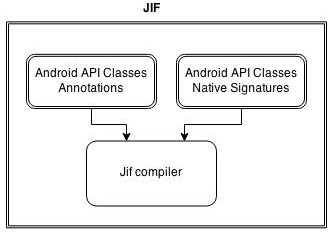
\includegraphics[width=5cm]{desingSol-steps1.jpg}
% 	\end{center}
% 	\caption{Tipos de anotación necesarias para implementar la solución.}
% 	\label{fig:desingSol-steps1}
% \end{figure}
% 
% \begin{figure}[t!]
% 	\begin{center}
% 	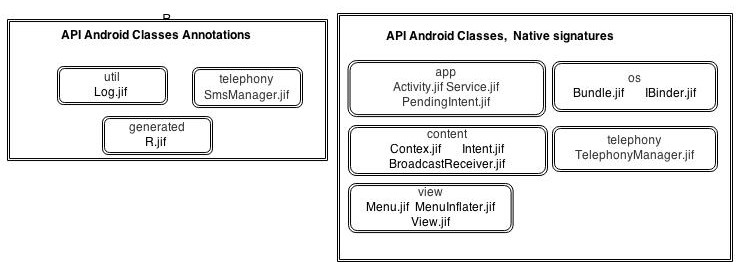
\includegraphics[width=12cm]{desingSol-step1-details.jpg}
% 	\end{center}
% 	\caption{Clases de la API a anotar.}
% 	\label{fig:desingSol-details}
% \end{figure}
% 
% El compilador de Jif tiene implementadas mediante el sistema de anotaciones Jif,
% las clases estándar del lenguaje Java para las que brinda soporte.\newline
% Ahora, para incluir clases Java ya existentes es posible recurrir a signaturas
% nativas, con las cuales se implementa la versión Jif de las clases fuentes, esto
% es, declarando constructores y cuerpo de los métodos a utilizar.
% 
% Para dar soporte a clases específicas de la API de Android se recurre a ambas
% opciones de anotación. Tal como se ilustra en la figura
% \ref{fig:desingSol-steps1}.\newline 
% El criterio para decidir que se anota de una u otra forma, depende de lo que
% represente la clase Android para verificar la política de seguridad
% establecida.\newline
% Las clases Log y SmsManager, que representan canales para conocer información,
% son anotadas de forma no nativa.\newline
% La opción de anotación nativa se utiliza
% para librerías Android, por ejemplo la clase TelephonyManager necesaria para utilizar
% el método getDeviceId.\newline
% En la figura \ref{fig:desingSol-details} se
% especifican clases de la API Android a anotar.\newline

\subsection{Descripción implementación}
Como se describió anteriormente, la implementación del diseño requiere
anotaciones a la API de Android y anotaciones en los aplicativos a
analizar.\newline 
En el caso de las anotaciones requeridas para la API, su
implementación se hace manualmente.\newline
En el caso de las anotaciones en el aplicativo a analizar, para lo
cual se propuso un esquema de anotación automatizable, se implementa un
prototipo de anotación en lenguaje Java. En la sección \ref{sec:diagramaClass}
de los anexos, se incluye su respectivo diagrama de clases.\newline
El anotador consta de cinco clases: Main, Source, XmlExtract, Annotation y
BufferWriter. 
En la clase Main se coordinan todos los pasos de anotación, así, la clase
Sources  identifica qué variable sources contiene la aplicación que se está
analizando; la clase Source  se apoya en la clase XmlExtract  para
identificar el source EdidText cuando el campo UI al que referencia corresponde
a un tipo textPassword. Como las interfaces UI se describen mediante XML, es
necesario extraer los datos de la interfaz con parsers XML.\\
Con la clase Annotation  se identifican y anotan los diferentes tipos de
métodos(métodos source, no source y métodos a sobreescribir).
En la clase BufferWriter  se anotan las variables sources, y finalmente se
retorna la versión .jif del aplicativo que se está analizando.\newline 
Para la anotación del código se utiliza la librería Java Parser 1.8  que permite
generar y visitar el árbol de sintaxis para la estructura del código de cada
programa, haciendo posible la adición de los labels de seguridad respectivos.\\
(Incluir Figura)\newline
\label{subsec:anotador}
\begin{figure}[t!]
	\begin{center}
	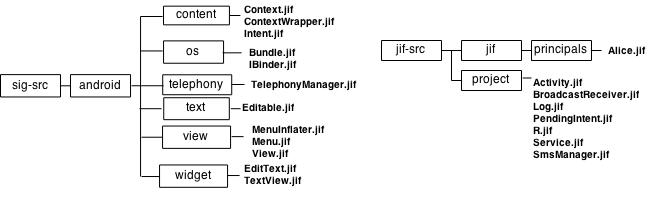
\includegraphics[width=12cm]{JifFilesystem.jpg}
	\end{center}
	\caption{Estructura de directorios en Jif.}
	\label{fig:jifFilesystem} 
\end{figure}

\subsection{Ambiente y herramientas}
\textit{Versión de la API de Android}\newline
Las anotaciones a las clases de la API Android y las aplicaciones a anotar
mediante el prototipo, corresponden a la versión Android 4.2.2(API Level 17).

\textit{Versión del compilador de Jif}\newline
El componente que verifica el cumplimiento de las políticas de seguridad,
corresponde a la versión 3.4.2 del compilador de Jif.

\textit{Estructura de trabajo en JIF}\newline
El compilador de Jif maneja una estructura de directorios en la que se incluye
el código fuente .jif de las aplicaciones a analizar. Como ilustra la figura
\ref{fig:jifFilesystem} se tienen los directorios principales sig-src y jif-src.
El directorio sig-src está destinado para incluir librerías adicionales.\newline 
El directorio jif-src contiene todo el código jif correspondiente al programa
como tal que se va evaluar mediante Jif. Para los propósitos del presente
trabajo, se tienen los subdirectorios principals y project. En el subdirectorio
principals se incluyen las autoridades requeridas, y en el subdirectorio
project se incluyen, tanto las clases específicas de los aplicativos Android a
analizar, como las clases de que estos heredan como: Activity.jif, Service.jif,
etc.

\subsection{Compilación, integración y finalmente ejecución }
En \ref{sec:ejecutarPrototipo} se describen las instrucciones paso a paso de cómo
ejecutar el anotador, y cómo compilar los aplicativos a analizar mediante Jif.





















